% ****** Start of file apssamp.tex ******
%
%   This file is part of the APS files in the REVTeX 4.1 distribution.
%   Version 4.1r of REVTeX, August 2010
%
%   Copyright (c) 2009, 2010 The American Physical Society.
%
%   See the REVTeX 4 README file for restrictions and more information.
%
% TeX'ing this file requires that you have AMS-LaTeX 2.0 installed
% as well as the rest of the prerequisites for REVTeX 4.1
%
% See the REVTeX 4 README file
% It also requires running BibTeX. The commands are as follows:
%
%  1)  latex apssamp.tex
%  2)  bibtex apssamp
%  3)  latex apssamp.tex
%  4)  latex apssamp.tex
%
\documentclass[%
 %reprint,
%superscriptaddress,
%groupedaddress,
%unsortedaddress,
%runinaddress,
%frontmatterverbose, 
%preprint,
%showpacs,preprintnumbers,
%nofootinbib,
%nobibnotes,
%bibnotes,
 amsmath,amssymb,
 aps,
 twocolumn,
%pra,
%prb,
%rmp,
%prstab,
%prstper,
%floatfix,
]{revtex4-1}

\usepackage{graphicx}% Include figure files
\usepackage{dcolumn}% Align table columns on decimal point
\usepackage{bm}% bold math
%\usepackage{hyperref}% add hypertext capabilities
%\usepackage[mathlines]{lineno}% Enable numbering of text and display math
%\linenumbers\relax % Commence numbering lines

%\usepackage[showframe,%Uncomment any one of the following lines to test 
%%scale=0.7, marginratio={1:1, 2:3}, ignoreall,% default settings
%%text={7in,10in},centering,
%%margin=1.5in,
%%total={6.5in,8.75in}, top=1.2in, left=0.9in, includefoot,
%%height=10in,a5paper,hmargin={3cm,0.8in},
%]{geometry}

\begin{document}

\preprint{APS/123-QED}

\title{Matching Matched Filtering with Deep Networks in Gravitational wave Astronomy}% Force line breaks with \\

\author{Hunter Gabbard}%Lines break automatically or can be forced with \\
 \email{Corresponding Author: h.gabbard.1@research.gla.ac.uk}
\author{Fergus Hayes}
\author{Michael Williams}%
\author{Chris Messenger}
\affiliation{%
 SUPA, School of Physics and Astronomy, \\
 University of Glasgow, \\
 Glasgow G12 8QQ, United Kingdom \\
}%

\date{\today}% It is always \today, today,
             %  but any date may be explicitly specified

\begin{abstract}
 We report a new method for classifying gravitational-wave (GW) signals from binary black holes (BBH) using a deep convolutional neural network. Using only the raw time series as input, we are able to distinguish GW signals injected in Gaussian noise from purely Gaussian noise time series with (\textbf{need figure of merit here}) percent accuracy. We compare our results with the standard method of matched filtering used in Advanced LIGO and find the methods to be comparable.  
\begin{description}
\item[Usage]
Secondary publications and information retrieval purposes.
\item[PACS numbers]
May be entered using the \verb+\pacs{#1}+ command.
\end{description}
\end{abstract}

\pacs{Valid PACS appear here}% PACS, the Physics and Astronomy
                             % Classification Scheme.
%\keywords{Suggested keywords}%Use showkeys class option if keyword
                              %display desired
\maketitle

%\tableofcontents


% You should probably mention matched filtering in more detail at some point in the introduction ...

\textit{Introduction} --- The field of gravitational wave astronomy has seen an explosion of binary black hole detections over the past several years [\textbf{cite detection papers}]. These detections were made possible by the Advanced Laser Interferometer Gravitational wave Observatory (aLIGO) detectors, as well as the recent joint detection of GW170814 with Advanced Virgo [\textbf{citation needed}]. Over the coming years many more such observations, including other more exotic sources such as binary neutron star (BNS), intermediate black hole (IMBH), and neutron star black hole (NSBH) mergers, are likely to be observed on a more frequent basis. As such, the need for more efficient search methods will be more pertinent as the detectors increase in \textit{volume} $\times$ \textit{time} sensitivity.

The search pipelines used to make these detections [\textbf{cite Usman et al. and gstlal folks}] are computationally expensive to run. Part of the reason being that the methods used by these \textit{search pipelines} are complex processes run over a large parameter space using advanced signal processing techniques. Distinguishing noise from signal in this search pipeline, and others like it, is done using a technique called matched template filtering. Matched template filtering uses a \textit{bank} of template waveforms that spans the astrophysical parameter space [\textbf{provide shit-ton of citations for this}] because we do not know \textit{a priori} what the parameters of the gravitational waves in the data are. Because the waveforms of the signals are well modeled, the pipeline uses matched filtering to search for those signals burried in the detector noise. More on how we implement this technique in comparisons with our model will be mentioned later in the methods section of this letter.

We propose that a deep learning algorithm which requires only the raw data time series as input with minimum signal processing would be one alternative. This pipeline could be pretrained and then run on real-time detector data with maximum efficiency and in low-latency.

Deep learning is a subset of machine learning which has gained in popularity over the past several years [\textbf{cite various successful nn's}]. A deep learning algorithm is composed of neurons which can be anywhere from one to several layers deep. Deep learning algorithms consists of an input layer, followed by one to several hidden layers and then one neuron that outputs a single value. This value can then either be used to solve classfication, or regression-like problems. 

In our model, we use a variant of a deep learning algorithm called a convolutional neural network (CNN) [\textbf{citation required}]. CNN layers are composed of five primary variants: input, convolutional, ReLu, pooling, and fully-connected. Where input holds the raw pixel values of the sample image, the convultional layer computes the dot product between the kernel and a local region of the input layer volume, ReLu applies an elementwise activation function leaving the size of the previous layer's output volume unchanged, pooling performs a downsampling operation along the spatial dimensions, and the fully-connected layer computes the class scores. 

In the following sections we will discuss our choice of network archetecture and tuning of it's hyperparameters, compare the results of our network with the widely used GW signal classification technique called matched filtering, and comment on future improvements related to this work.      

\textit{Methods} --- In this analysis, in order to make the problem simple, we only distinguish between BBH signals injected into a Gaussian noise time series and pure white Gaussian noise time series. The time series for both classes of signals are 1s in duration sampled at 8192 Hz. \textbf{say more about how noise and injection are generated using Chris's code.} 

For our noise signals we generate a power spectrum density (PSD) that is comparable to aLIGO design sensitivity [\textbf{perhaps cite lal folks}]. That PSD is then converted to an amplitude time series where a random phase shift is given to each spectral component. The inverse real fast fourier transform (IFFT) is then applied and returns a Gaussian time series.

Injections are made using the IMRPhenomD type waveform [\textbf{cite Phenom wf paper}] where the component masses of the waveform range from 5\(M_\odot\) to 100\(M_\odot\) (\textbf{not sure if correct?}). 

\begin{table*}[]
\centering
\caption{The optimal network structure (seen below) was determined through multiple tests and tunnings of hyperparameters by means of trial and error. The network consists of 8 convolutional layers, followed by 2 fully-connected layers. Max-pooling is performed on the first, fifth, and eigth layer, whereas dropout is only performed on the two fully-connected layers. Each layer uses an Elu activation function while the last layer uses a Softmax activation function in order to normalize the output values to be between zero and one so as to give a probability value for each class. \\} 
\label{my-label}
\begin{tabular}{lllllllllll}
                    & layer 1 & layer 2 & layer 3 & layer 4 & layer 5 & layer 6 & layer 7 & layer 8 & layer 9 & layer 10 \\
Number of Kernals   & 8       & 16      & 16      & 32      & 64      & 64      & 128     & 128     & 64      & 2        \\
Filter Size         & 32      & 16      & 16      & 16      & 8       & 8       & 4       & 4       & n/a     & n/a      \\
Max Pooling         & 8       & 1       & 1       & 1       & 6       & 1       & 1       & 4       & n/a     & n/a      \\
Fully Connected     & n/a     & n/a     & n/a     & n/a     & n/a     & n/a     & n/a     & n/a     & yes     & yes      \\
Drop out            & 0.0     & 0.0     & 0.0     & 0.0     & 0.0     & 0.0     & 0.0     & 0.0     & 0.5     & 0.5      \\
Activation Function & Elu     & Elu     & Elu     & Elu     & Elu     & Elu     & Elu     & Elu     & Elu     & Softmax 
\end{tabular}
\end{table*}

The samples are then arranged in the form of a $1 \times 8192$ pixel sample which is scaled by the GW strain amplitude, $h(t)$, over one color channel (grayscale). (\textbf{give ligo definition of optimal SNR})

\textit{Results} --- In this case, we cyclically adjust the learning rate to oscialte between $5 \times 10^{-4}$ and $1 \times 10^{-3}$ at a constant frequency. Studies have shown that this policy of learning rate adjustement (\textbf{blah blah blah})

\begin{figure*}[]
 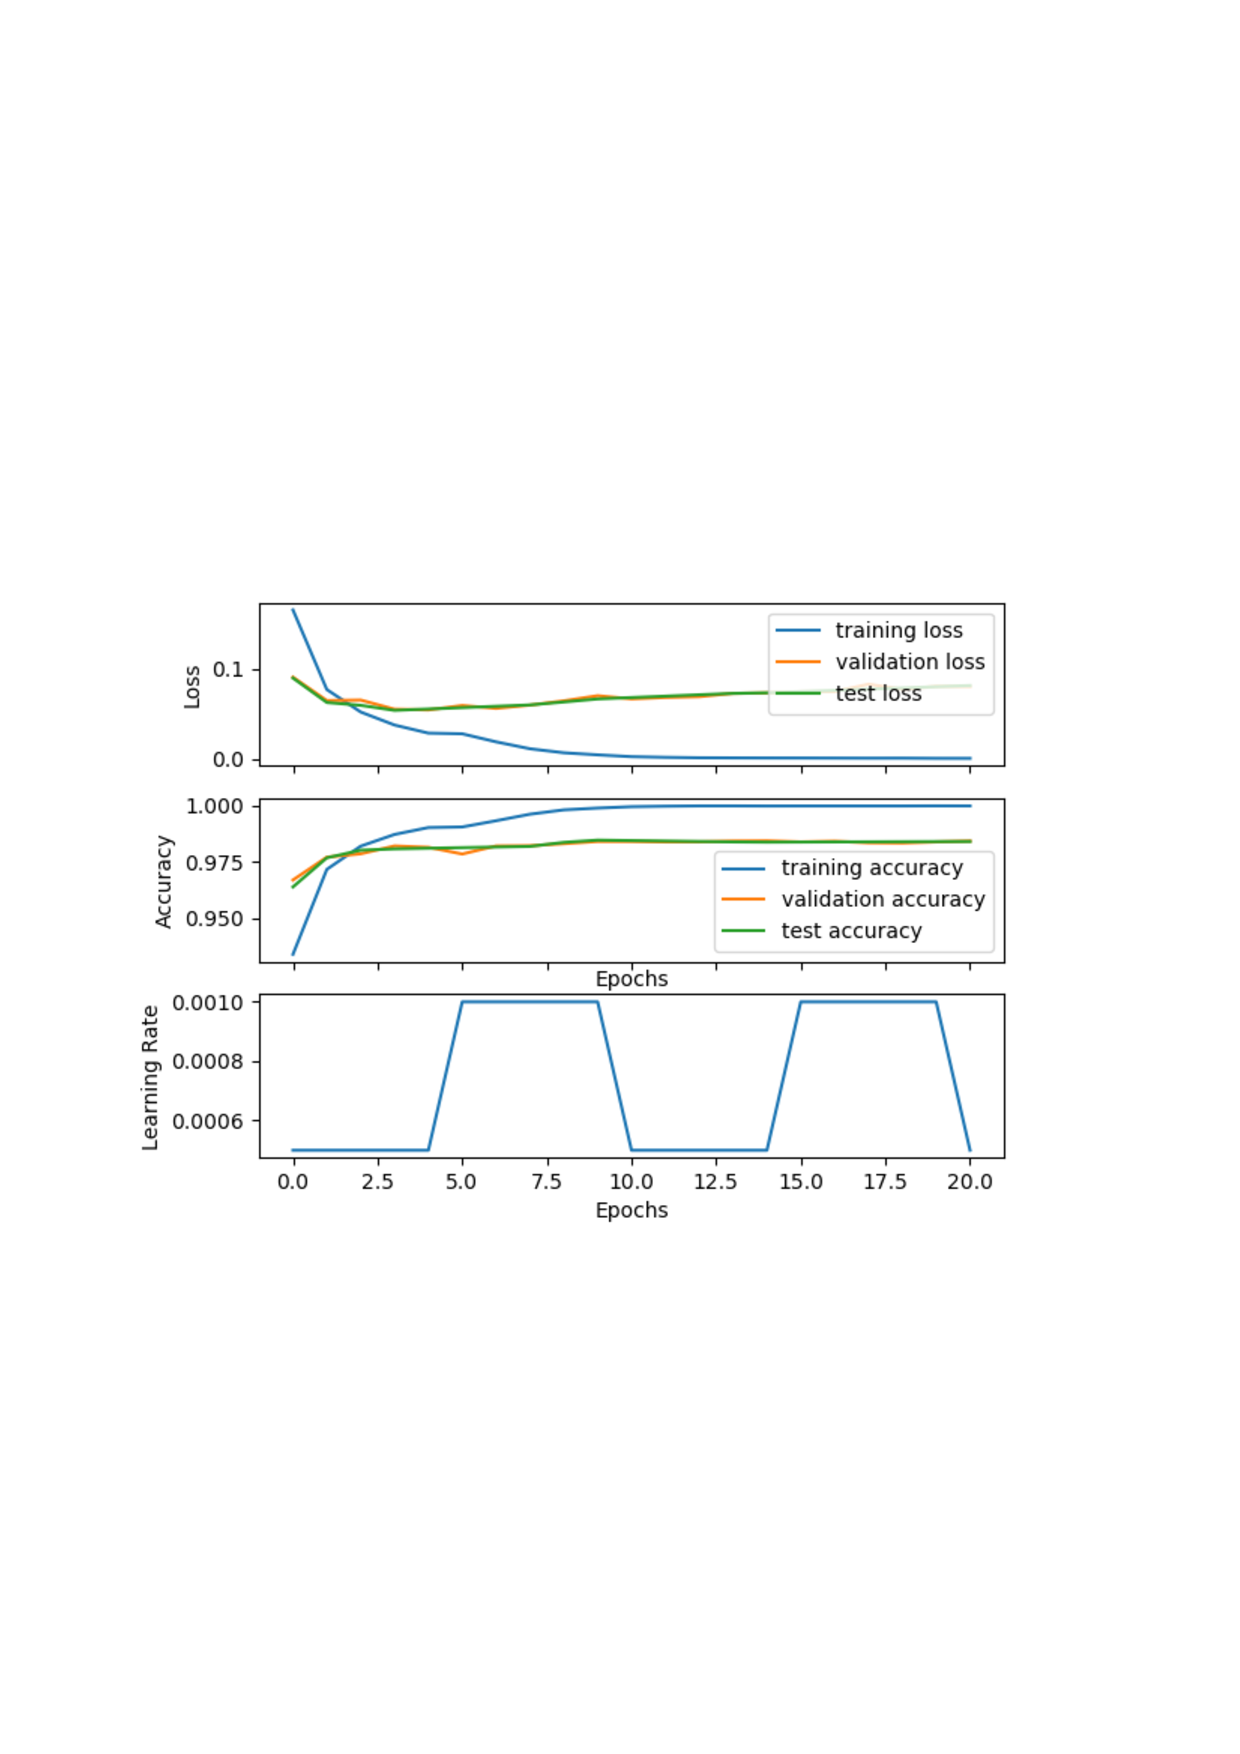
\includegraphics[width=0.5\textwidth]
 {figures/loss.png}
 \caption{\label{fig:loss curve ex} The loss, accuracy and learning rate plots (shown above) illustrate how the network's performance is defined as a function of the number of training epochs. The goal is to minimize the loss function, which will in turn maximize the accuracy of the classifier. The first initial epochs see an exponential decrease in the loss function and then a slowly falling monotonic curve to follow. This indicates that the longer our network is trained, a limit with respect to the accuracy is approached.}
\end{figure*}

\begin{figure*}[]
 \centering
  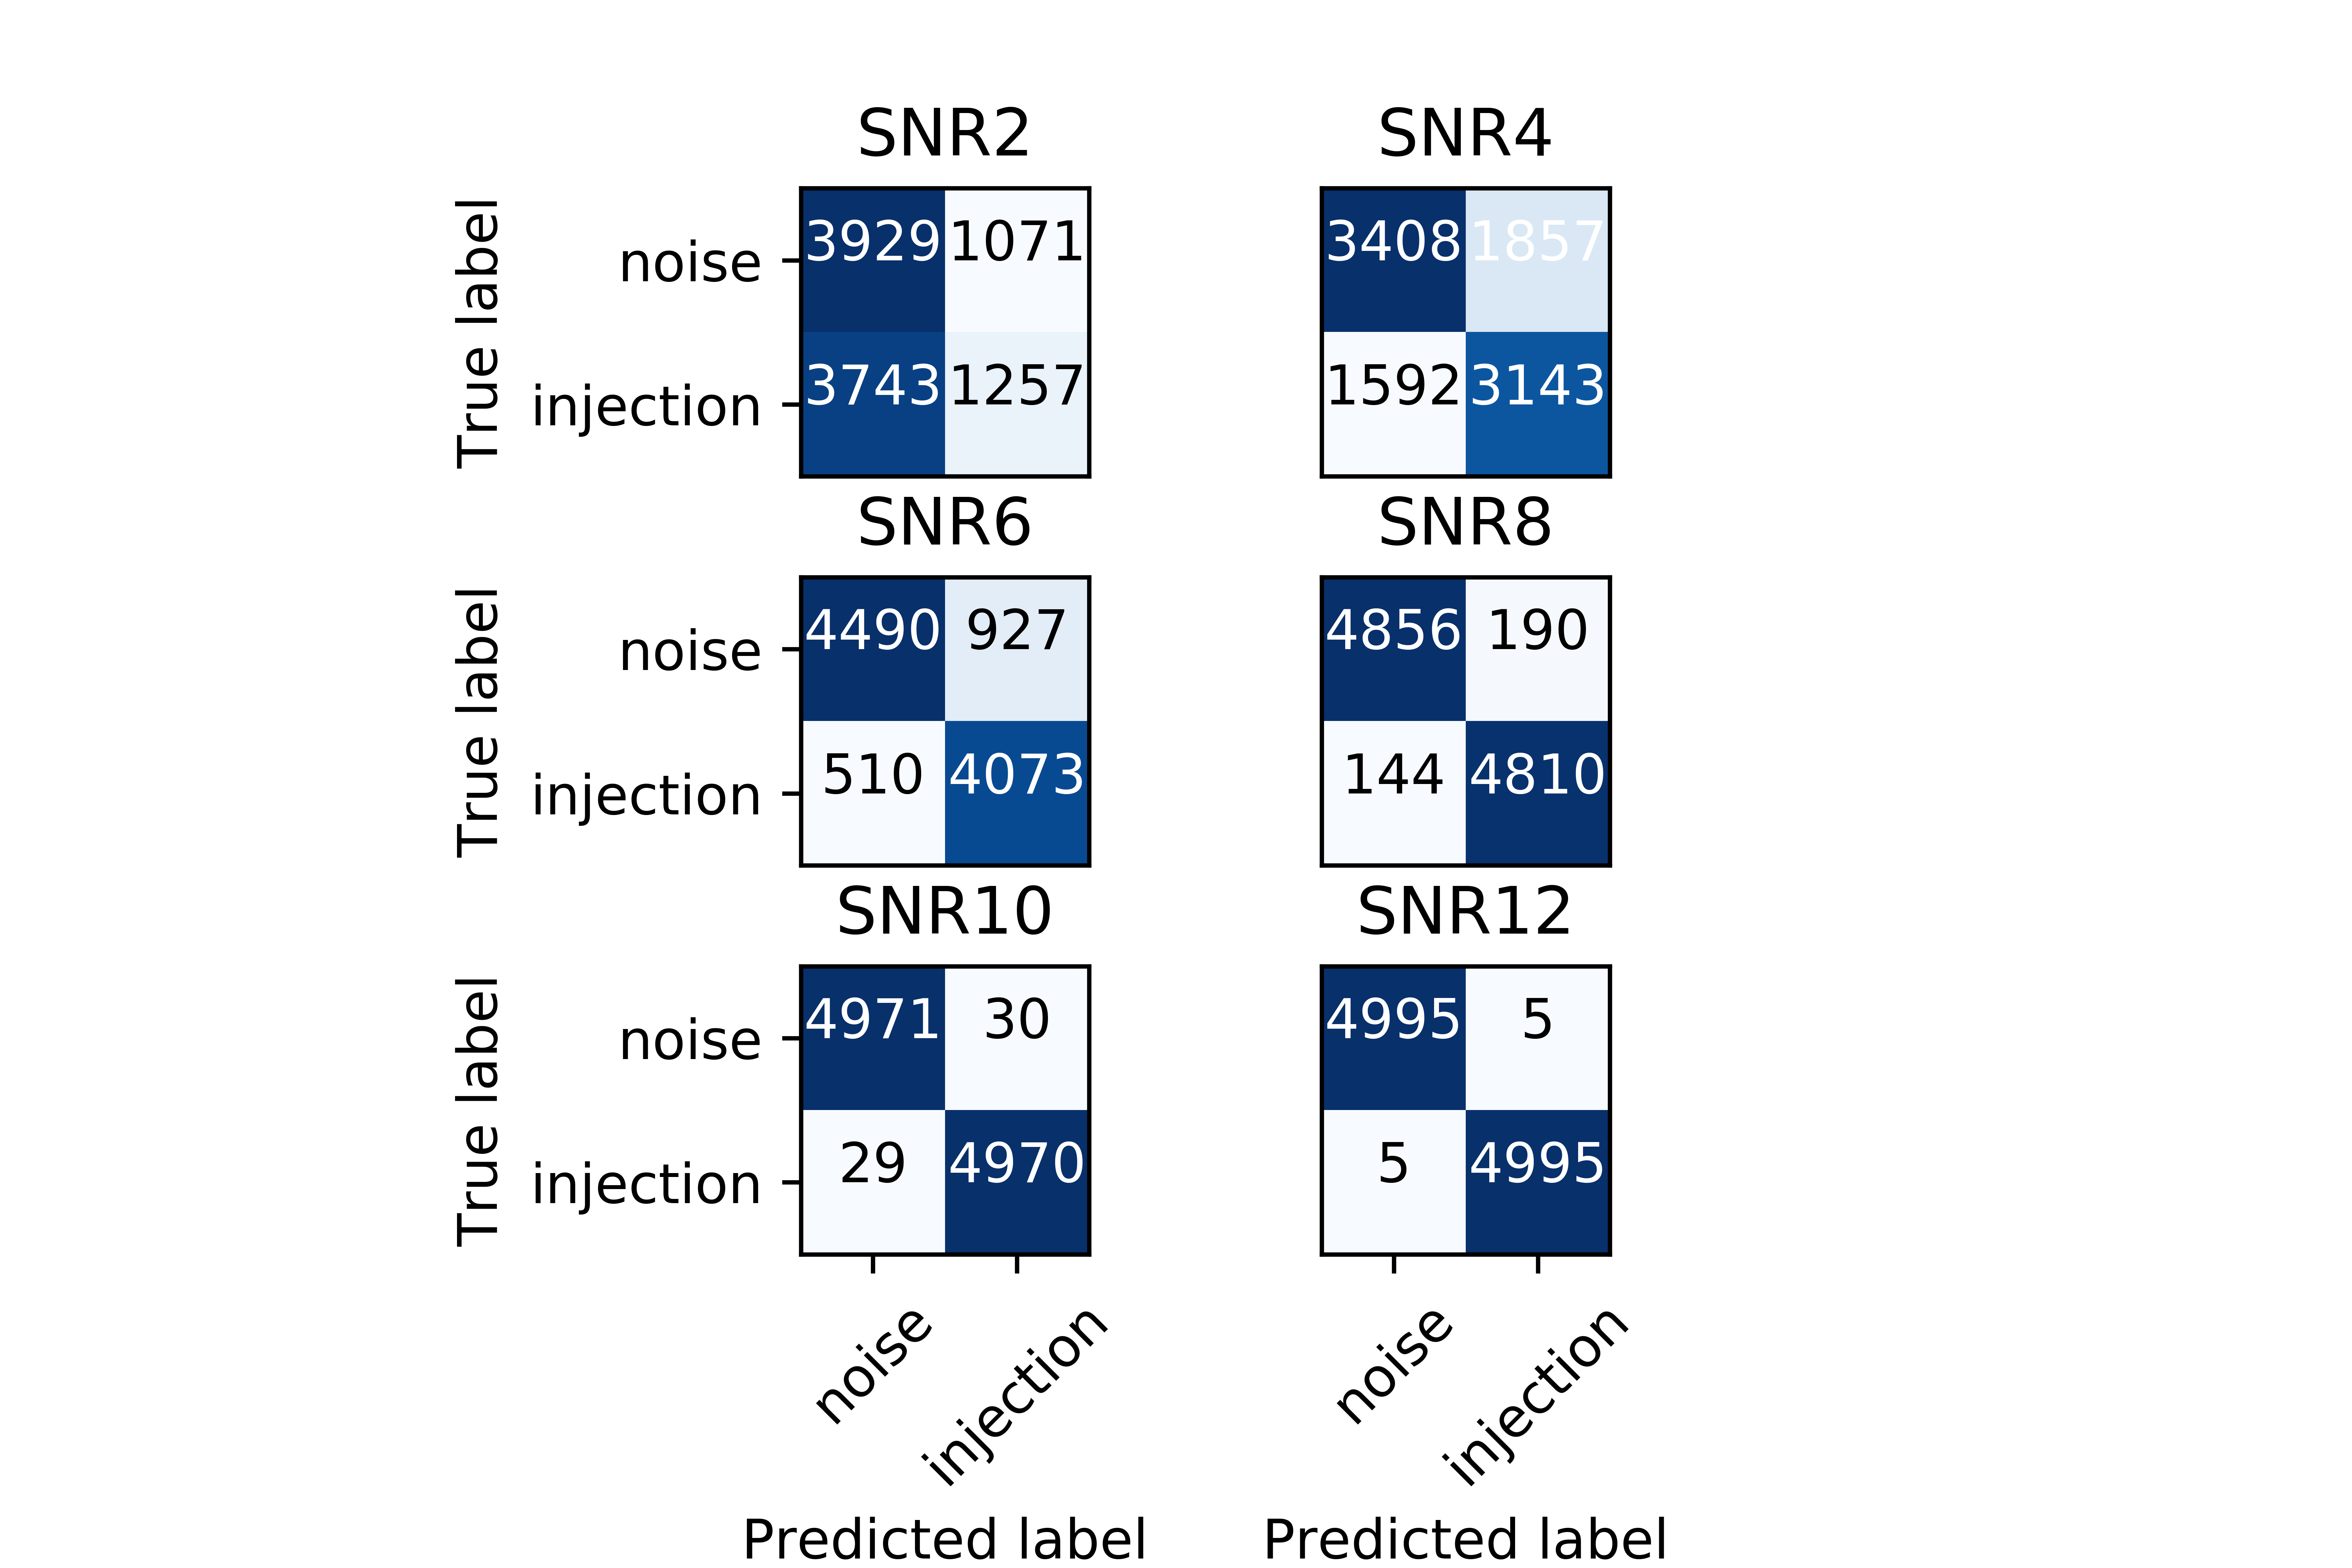
\includegraphics[width=0.5\textwidth]
 {figures/confusion_matrix.png}
 \caption{\label{fig:confusion} Say something about confusion matrix here.}
\end{figure*}

\begin{figure*}[]
 \includegraphics[width=0.5\textwidth]
 {figures/acc_both_0_01_up.png}
 \caption{\label{fig:accuracy} \textbf{Need this plot but without the references to GH.}}
\end{figure*}

\begin{figure*}[]
 \includegraphics[width=0.5\textwidth]
 {figures/ROC_curves_both_up.png}
 \caption{\label{fig: ROC curve} \textbf{Need this plot but without references to GH.}}
\end{figure*}

\textit{Conclusions} --- 



% The \nocite command causes all entries in a bibliography to be printed out
% whether or not they are actually referenced in the text. This is appropriate
% for the sample file to show the different styles of references, but authors
% most likely will not want to use it.
\nocite{*}

\bibliography{apssamp}% Produces the bibliography via BibTeX.

\end{document}
%
% ****** End of file apssamp.tex ******
